\section{Durchführung}
\label{sec:Durchführung}

\subsection{Versuchsaufbau}

Zur expliziten Messung wird die Messapparatur \autoref{fig:abb2} entsprechend aufgebaut.

\begin{figure}[H]
    \centering
    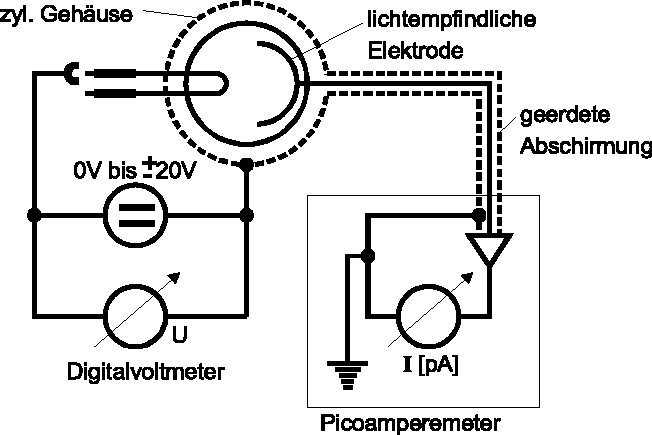
\includegraphics[width=0.75\textwidth]{figures/Abb2.pdf}
    \caption{Schaltbild zur verwendeten Messapparatur \cite{ap10}.}
    \label{fig:abb2}
\end{figure}

Die dabei verwendete Photozelle ist in \autoref{fig:abb3} näher zu erkennen.

\begin{figure}[H]
    \centering
    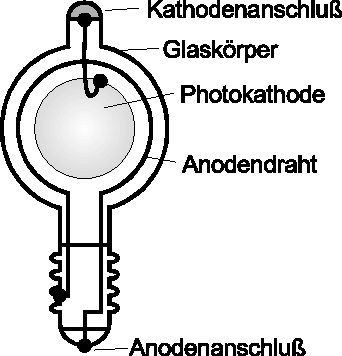
\includegraphics[width=0.3\textwidth]{figures/Abb3.pdf}
    \caption{Verwendete Photozelle in schematischer Darstellung \cite{ap10}.}
    \label{fig:abb3}
\end{figure}

Die Photozelle ist in einen evakuierten Glaskörper eingeschlossen, eine aufgedampfte Metalloberfläche übernimmt dabei die Rolle der Kathode, der parallel zur Kathode ausgerichtete Drahtring ist dabei die Anode. \\

Damit nun mit monochromatischem, aber verschiedenem Licht gearbeitet werden kann, wird der in \autoref{fig:abb5} dargestellte Aufbau vor der eigentlichen Apparatur aufgebaut.

\begin{figure}[H]
    \centering
    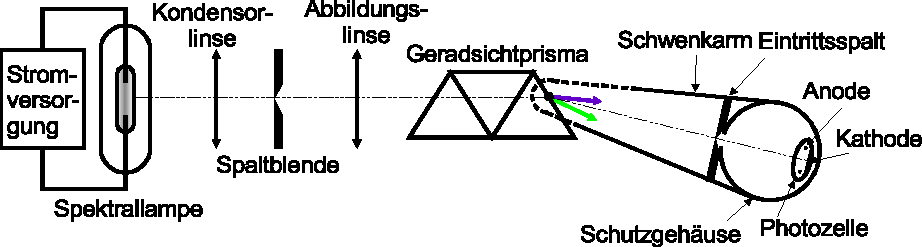
\includegraphics{figures/Abb5.pdf}
    \caption{Schematische Darstellung des Aufbaus zur Aufspaltung des Lichts \cite{ap10}.}
    \label{fig:abb5}
\end{figure}

Die Hg-Spektrallampe emittiert dabei Licht bestimmter diskreter Wellenlängen, die über die Linsen und die Blende fokussiert und mithilfe des Prismas aufgespalten werden.


\subsection{Versuchsdurchführung}

Zunächst muss der Aufbau justiert werden.
Dazu werden die Abstände zwischen den einzelnen Linsen so verändert, dass möglichst scharfe Spektrallinien zu erkennen sind. \\

Für fünf verschiedene Spektrallinien, also fünf verschiedene Wellenlängen wird nun der Photostrom in Abhängigkeit der Bremsspannung gemessen.
Das Messintervall wird dabei auf $0 \,\unit{\volt} \leq U \leq U_\text{g}$, es wird also gemessen, bis kein Photostrom mehr auftritt. \\

Speziell für Licht der Wellenlänge $\lambda = 578 \, \unit{\nano\meter}$ wird eine Kennlinie aufgenommen.
Dazu wird die Spannung im Intervall $-U_\text{g} \leq U \leq 20 \,\unit{\volt}$ variiert und der Photostrom $I_\text{Ph}$ aufgenommen.

